\documentclass[14pt,t]{beamer}
\usepackage{fontspec}
\usepackage{color}
\usepackage{minted}

%% These fonts are non-free.
%% Comment out the lines if you don't have them.
\setmainfont{Equity Text A}
\setsansfont{Concourse T3}
\setmonofont{Triplicate T4}

\definecolor{bgcolor}{RGB}{20,25,28}
\definecolor{codecolor}{RGB}{249,38,114}
\hypersetup{colorlinks,linkcolor=,urlcolor=codecolor}
\setbeamercolor{background canvas}{bg=bgcolor}
\setbeamercolor{normal text}{fg=white}
\setbeamercolor{itemize item}{fg=lightgray}
\setbeamercolor{enumerate item}{fg=lightgray}
\setbeamertemplate{itemize items}[circle]
\setbeamertemplate{navigation symbols}{}
%% These styles are kinda annoying the fuck outta me
%% If I have a change of heart (again), then here's the
%% file to edit:
%% /usr/lib/python3.6/site-packages/pygments/styles/monokai.py
%% Don't forget to remove the _minted* dir afterwards.
\usemintedstyle{monokai}
\newminted[lispcode]{common-lisp}{fontsize=\footnotesize}
\newminted[htmlcode]{html}{fontsize=\footnotesize}
\def\code#1{{\color{codecolor}\texttt{#1}}}

\renewcommand{\theFancyVerbLine}{\color{darkgray}\large \oldstylenums{\arabic{FancyVerbLine}}}
\renewcommand{\title}[1]{
  {\huge #1} \vskip 0.4cm
}
\renewcommand{\subtitle}[1]{
  \vskip 0.3cm {\Large #1} \vskip 0.2cm %
}

\begin{document}
\begin{frame}
  \begin{center}
    
\includegraphics[height=4cm]{avatar.png}\\
    \vspace{0.2cm}
    {\LARGE Nicolas Hafner} \\
    \vspace{0.2cm}
    {\Large @Shinmera} \\
    \vspace{0.2cm}
    \url{https://everything.shinmera.com}
  \end{center}
\end{frame}

\begin{frame}
  \begin{center}
    
\includegraphics[width=0.8\columnwidth]{radiance.png}
  \end{center}
\end{frame}

\begin{frame}
  \title{About Seven Years Ago}
  \begin{center}
    
\includegraphics[width=0.8\columnwidth]{baby-at-computer.jpg}
  \end{center}
\end{frame}

\begin{frame}
  \title{About Seven Years Ago}
  \begin{itemize}
  \item Comics with comments
  \item Forums for discussions
  \item How not to require users to have multiple logins?
  \item Write my own software \pause ... in PHP
  \end{itemize}
\end{frame}

\begin{frame}
  \title{Radiance Goals}
  \begin{itemize}
  \item ``Do it right this time''
  \item Run multiple applications side-by-side
  \item Share resources between applications
  \item Make as many parts optional as possible
  \item Configurable by administrator
  \item Documented well and easy to use
  \end{itemize}
\end{frame}

\begin{frame}
  \title{Radiance Problems}
  \begin{enumerate}
  \item How to make features optional and exchangeable
  \item How to divide up URL address space
  \item How to make deployment as easy as possible
  \end{enumerate}
\end{frame}

\begin{frame}
  \title{1. Interfaces}
  \begin{itemize}
  \item Standardise access to common features
  \item Load interface implementation on demand
  \end{itemize}
\end{frame}

\begin{frame}[fragile]
  \title{Interface Definition}
\begin{lispcode}
(define-interface cache
  (defun invalidate (name)
    "Causes the cached value to be re-computed.")

  (defmacro with-caching (name test &body body)
    "Caches the return value if TEST is non-NIL."))
\end{lispcode}
\end{frame}

\begin{frame}[fragile]
  \title{Interface Usage}
\begin{lispcode}
(asdf:defsystem another-todo-app
  :components ((:file "todo.lisp"))
  :depends-on ((:interface :cache)))
\end{lispcode}
  \pause
  \vskip 1cm
  {\footnotesize\code{todo.lisp}}
\begin{lispcode}
(defun render-todo-list (user)
  (cache:with-caching (user (changes-made-p user))
    (render-template (template "todo-list.html")
                     (fetch-todo-items user))))
\end{lispcode}
\end{frame}

\begin{frame}[fragile]
  \title{Interface Implementation}
\begin{lispcode}
(asdf:defsystem my-cache
  :components ((:file "impl.lisp")))
\end{lispcode}
  \vskip 1cm
  {\footnotesize\code{impl.lisp}}
\begin{lispcode}
(defvar cache::*caches* (make-hash-table))

(defun cache:invalidate (name)
  (remhash name *caches*))

(defmacro cache:with-caching (name test &body body)
  (once-only (name)
    `(or (and (not ,test) (gethash ,name *caches*))
         (setf (gethash ,name *caches*)
               (progn ,@body)))))
\end{lispcode}
\end{frame}

\begin{frame}
  \title{Interface Advantages}
  \begin{itemize}
  \item No overhead as everything is direct calls
  \item Allows framework to grow or shrink as needed
  \item Implementation can be exchanged
  \end{itemize}
\end{frame}

\begin{frame}
  \title{2. Routing}
  \begin{itemize}
  \item Find proper content to deliver on an address
  \item Share the address space between applications
  \end{itemize}
\end{frame}

\begin{frame}
  \title{Routing Life-Cycle}
  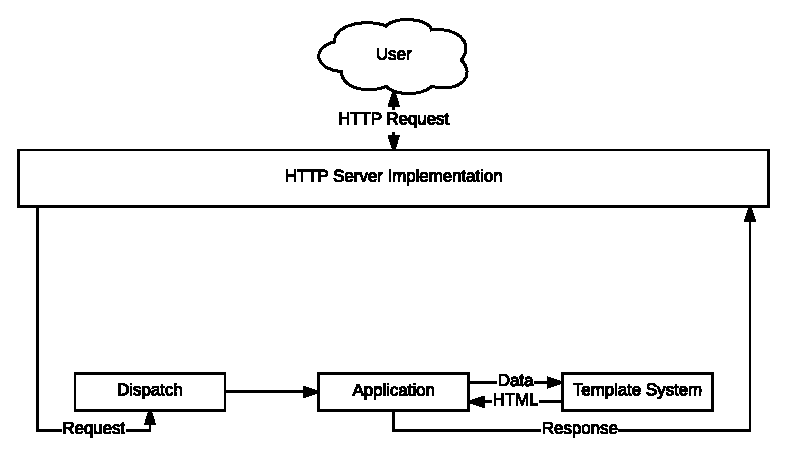
\includegraphics[width=\columnwidth]{request-simple}
\end{frame}

\begin{frame}
  \title{Routing Life-Cycle}
  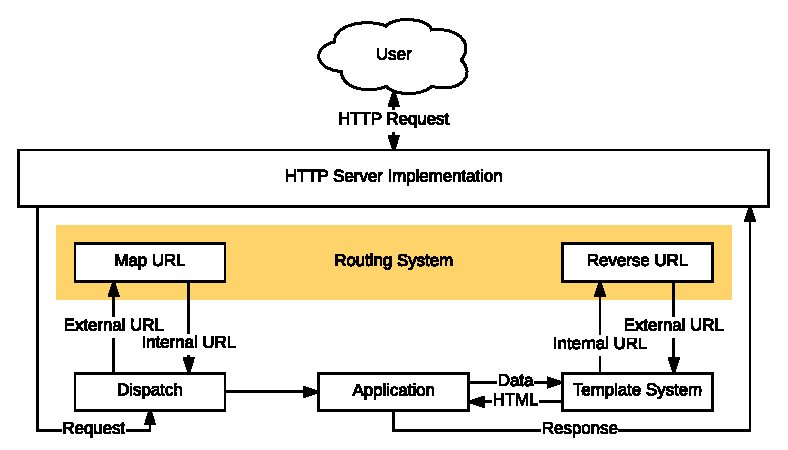
\includegraphics[width=\columnwidth]{request}
\end{frame}

\begin{frame}[fragile]
  \title{Page Definition}
\begin{lispcode}
(define-page add-page "todo/add" ()
  (render-template (template "todo-add.html")))
\end{lispcode}
  \pause
  \vskip 1cm
  {\footnotesize\code{todo-add.html}}
\begin{htmlcode}
<form method="post">
  <textarea name="text"></textarea>
  <input type="submit" @formaction="todo/submit" />
</form>
\end{htmlcode}
\end{frame}

\begin{frame}
  \title{Routing Example}
  Request \;\;\code{http://example.com/doit/add}
  \begin{enumerate}
  \item Map \code{example.com/doit/add} \\
    to \hskip0.5cm \code{todo/add}
  \item Dispatch to \code{add-page}
  \item Reverse \code{todo/submit} \\
    to \hskip1.1cm \code{example.com/doit/submit}
  \item Deliver compiled HTML
  \end{enumerate}
\end{frame}

\begin{frame}[fragile]
  \title{Route Definition}
\begin{lispcode}
(define-string-route todo :mapping
  "/doit/(.*)" "todo/\\1")

(define-string-route todo :reversal
  "todo/(.*)" "/doit/\\1")
\end{lispcode}
  \pause \vskip 1.0cm
\begin{lispcode}
(define-route todo :mapping (uri)
  (when (begins-with "doit/" (path uri))
    (setf (domains uri) '("todo")
          (path uri) (subseq (path uri) 5))))
\end{lispcode}
\end{frame}

\begin{frame}
  \title{Routing Advantages}
  \begin{itemize}
  \item Easier to visualise when developing
  \item URLs can be easily rewritten
  \item Arbitrary transforms by functions
  \end{itemize}
\end{frame}

\begin{frame}
  \title{3. Environments}
  \begin{itemize}
  \item Unify configuration of applications
  \item Ease setup for non-developers
  \end{itemize}
\end{frame}

\begin{frame}[fragile]
  \title{Configuring Interfaces}
\begin{lispcode}
(radiance:startup :my-env)

(setf (mconfig :radiance-core :interface :cache)
      "my-cache")
  ;=> "my-cache"
\end{lispcode}
  \pause
  \vskip 0.5cm
  {\footnotesize\code{my-env/radiance-core/radiance-core.conf.lisp}}
\begin{lispcode}
((:interfaces (:cache . "my-cache")
              ...)
 ...)
\end{lispcode}
  \pause
  \vskip 0.5cm
  {\footnotesize\code{repl}}
\begin{lispcode}
(ql:quickload :another-todo-app)
  ;=> Loading my-cache...
\end{lispcode}
\end{frame}

\begin{frame}[fragile]
  \title{Environment Access}
\begin{lispcode}
(in-package :another-todo-app)
(defvar *image-cache* (config-pathname "images/"))

(define-trigger startup ()
  (defaulted-config "Simple ToDo Lists" :title)
  (defaulted-config 256 :max-items))

(defun add-item (text user)
  (when (<= (config :max-items) (count-items user))
    (error "Too many items!"))
  ...)
\end{lispcode}
\end{frame}

\begin{frame}
  \title{Environment Advantages}
  \begin{itemize}
  \item Easy to switch between setups
  \item Config files for people with no Lisp knowledge
  \item Unified place for storage of files
  \end{itemize}
\end{frame}

\begin{frame}
  \title{Putting it All Together}
  \begin{itemize}
  \item Bulk of features provided through interfaces
  \item Features are pluggable, but standardised
    \pause \vskip 0.5cm
  \item Routing gives a convenient development view
  \item Setup is quick and relatively simple
    \pause \vskip 0.5cm
  \item Environments standardise file storage
  \item Unified configuration and setup
  \end{itemize}
\end{frame}

\begin{frame}
  \title{Existing Applications}
  \begin{itemize}
  \item Reader: A blog
  \item Purplish: An imageboard
  \item Filebox: A file storage
  \item Plaster: A paste service
  \item Chatlog: An IRC log viewer
  \end{itemize}
\end{frame}

\begin{frame}
  \title{Resources}
  \subtitle{Website}
  {\footnotesize\url{https://shirakumo.org/radiance}}
  \subtitle{Documentation}
  {\footnotesize\url{https://shirakumo.org/radiance/documentation}}
  \subtitle{Lengthy Tutorial}
  {\footnotesize\url{https://shirakumo.org/radiance/tutorial}}
  \subtitle{Existing Applications}
  {\footnotesize\url{https://github.com/shirakumo}}
\end{frame}

\begin{frame}
  \title{Acknowledgements}
  Thanks to Joram Schrijver, Till Ehrengruber, and Robert Strandh for feedback, corrections, and suggestions on the paper. Thanks to Joram, Till, and Janne Pakarinen for testing and feedback on Radiance.
\end{frame}

\end{document}

%%% Local Variables:
%%% mode: latex
%%% TeX-master: t
%%% TeX-engine: luatex
%%% TeX-command-extra-options: "-shell-escape"
%%% End:
